\documentclass[10pt]{beamer}
\usepackage{beamerthemesplit, amsmath, graphicx, bbm, multicol, multirow}

\usetheme{Berkeley}

\DeclareMathOperator*{\argmax}{argmax}
\DeclareMathOperator*{\argmin}{argmin}
\renewcommand{\baselinestretch}{1.2}

\title{Forward Price Simulation}
\author{Hao Wu}
\date{August 24, 2007}
\institute{Risk Management Group\\
Constellation Energy \& \\
Department of Biostatistics\\
Johns Hopkins School of Public Health}

\begin{document}

\frame{\titlepage}

%% overview page
\frame{
  \frametitle{Overview}
  \tableofcontents
}

%% motivation
\section{Background}

% motivation
\frame
{
  \frametitle{Motivation}
Long term price simulation is useful for:
\begin{itemize}
\item Potential Exposure
\item Asset valuation
\item Portfolio optimization
\end{itemize}
}

\frame
{
  \frametitle{Challenges}
\begin{itemize}
\item Simulation of 
a few correlated time series is trivial. 
\item Main challenge in 
this project is the scale of the data. 
\begin{itemize}
\item Around 650 curves (commodities)
\item 24 to 60 contract month for each curve
\item Correlations among 30,000 curve/month must be kept
\end{itemize}
\end{itemize}
}

%%%%%%%%%%%%%%%%%%%%%%%%%%%%%%%%%%%%%%%%%%%%%%%%
%% Data exploraion section
%%%%%%%%%%%%%%%%%%%%%%%%%%%%%%%%%%%%%%%%%%%%%%%%

\section{Data Exploration}

%%% NG data
\frame 
{
  \frametitle{Data Exploration}
Understand the historical data is crucial in forward simulation.
\begin{itemize}
\item Natural Gas, Coal, Oil
\item Electricity and its dependency on fuels
\item Volatility
\end{itemize}
}

\frame
{
  \frametitle{NG EXCHANGE historical prices} 
\begin{center}
  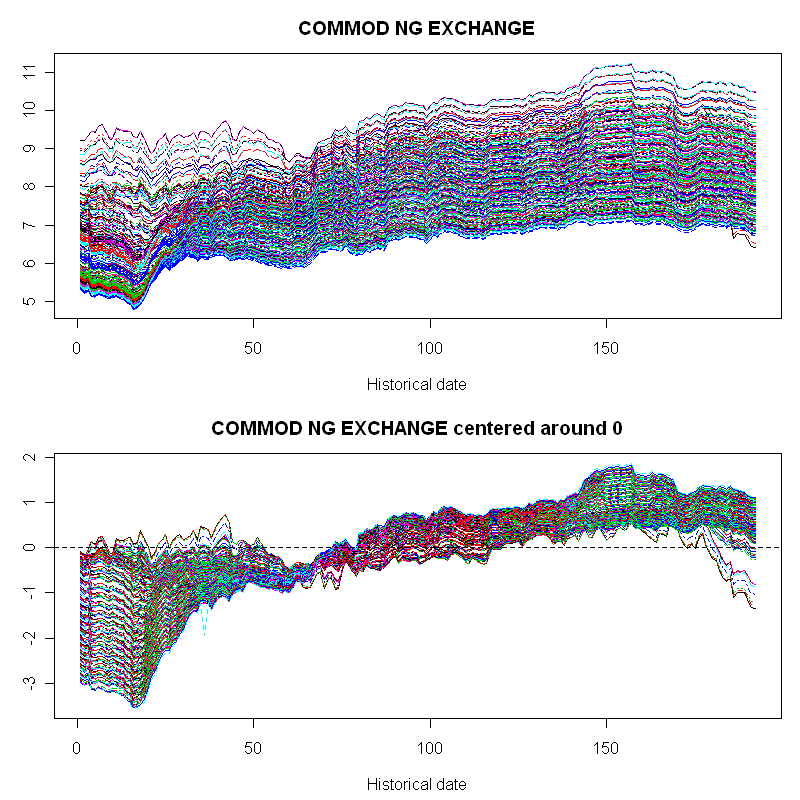
\includegraphics[height=2.5in]{figures/henry01.png}
\end{center}
}

\frame
{
  \frametitle{NG EXCHANGE  prices - January contracts} 
\begin{center}
  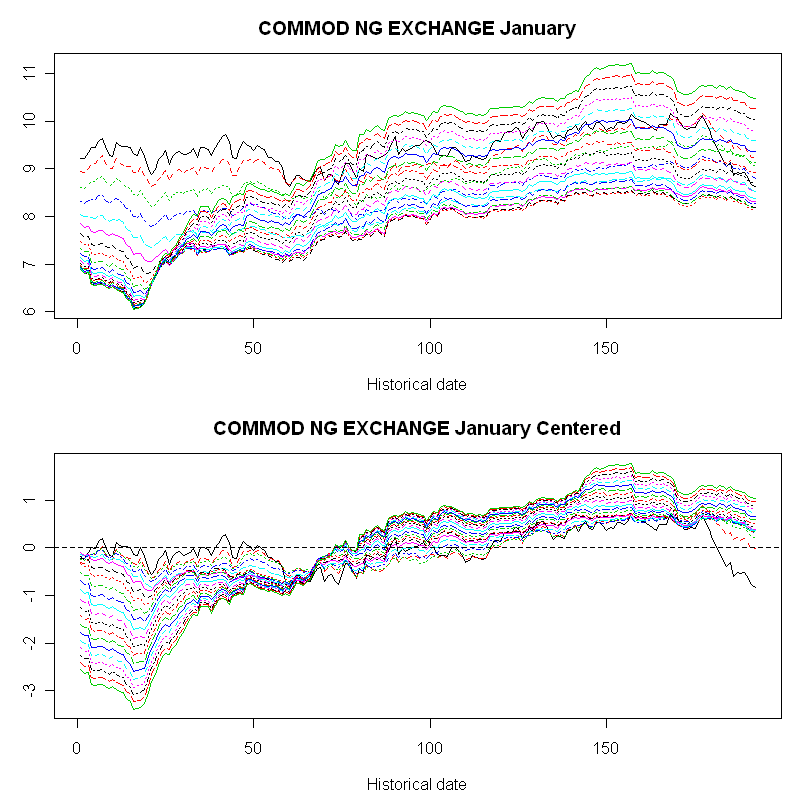
\includegraphics[height=2.5in]{figures/henry02.png}
\end{center}
}

\frame
{
  \frametitle{NG EXCHANGE  prices - August contracts} 
\begin{center}
  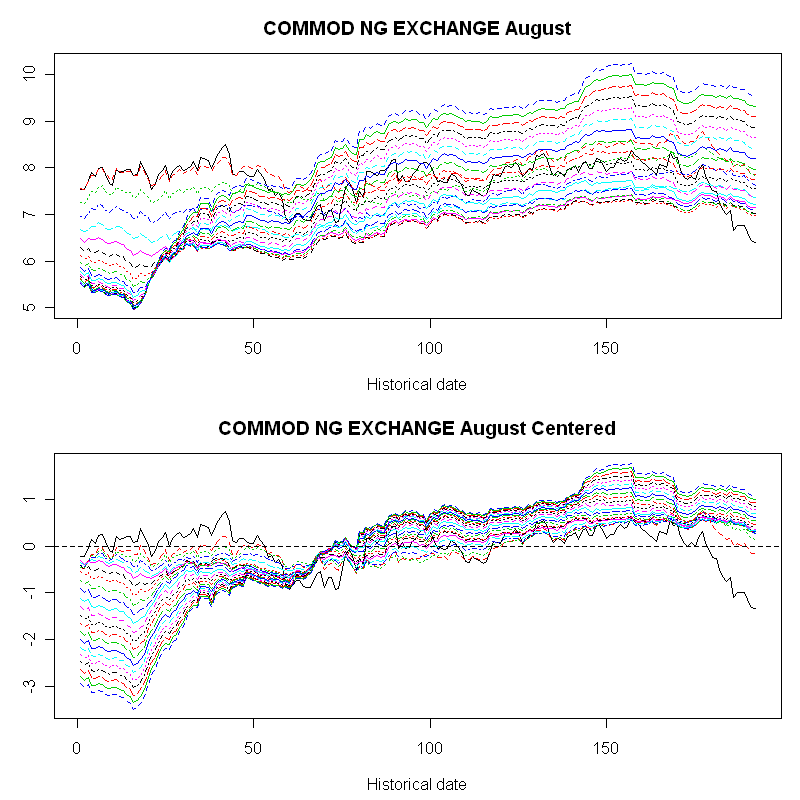
\includegraphics[height=2.5in]{figures/henry03.png}
\end{center}
}

\frame
{
  \frametitle{NG EXCHANGE historical prices by contract month } 
\begin{center}
  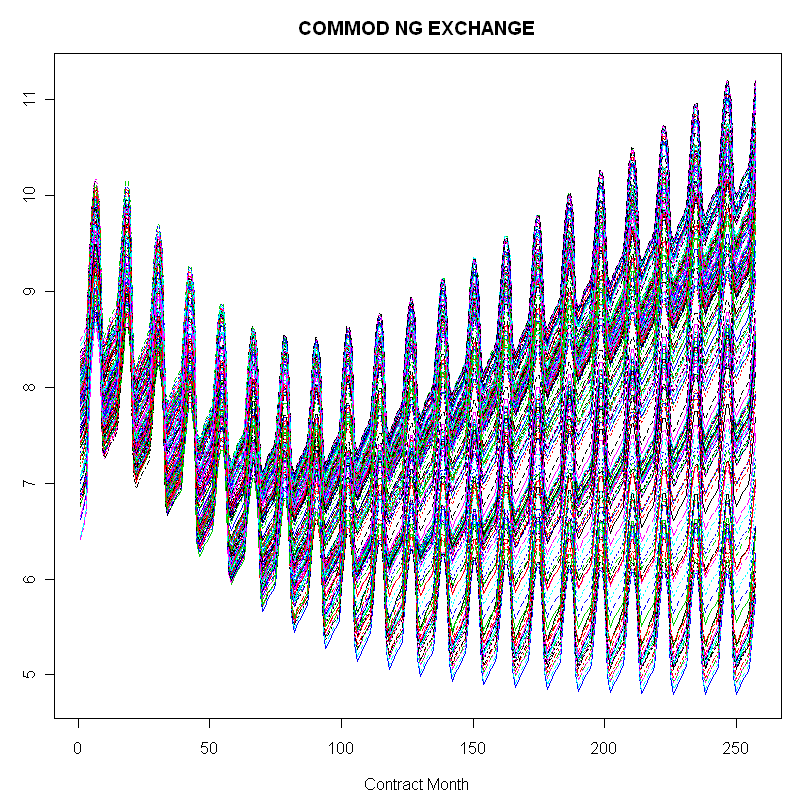
\includegraphics[height=2.5in]{figures/henry04.png}
\end{center}
}

\frame
{
  \frametitle{NG EXCHANGE prices by contract month - January contracts} 

\begin{center}
  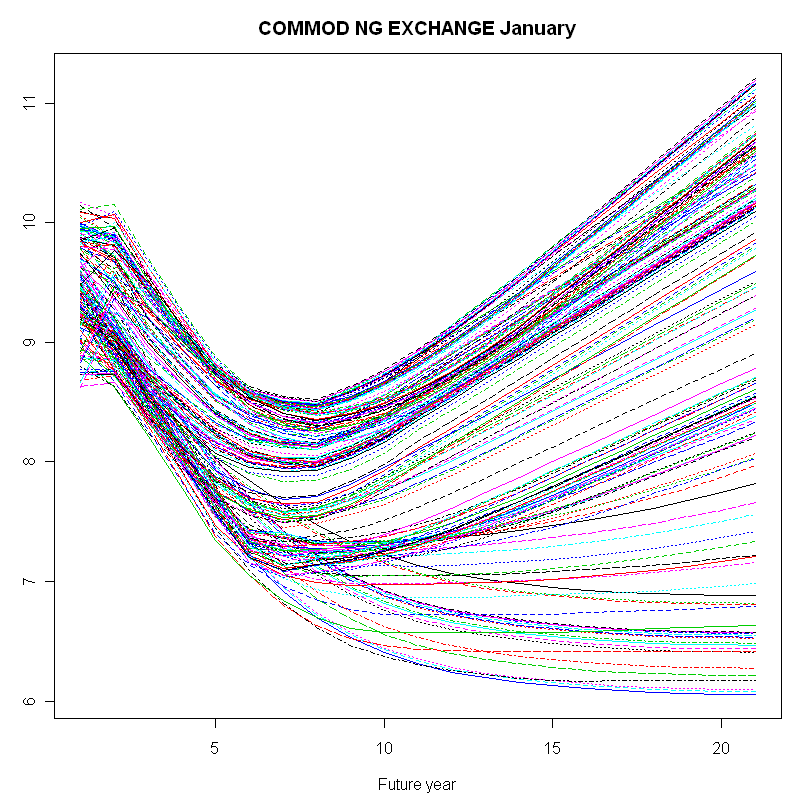
\includegraphics[height=2.5in]{figures/henry06.png}
\end{center}
}

\frame
{
  \frametitle{NG EXCHANGE  prices by contract month - August contracts} 
\begin{center}
  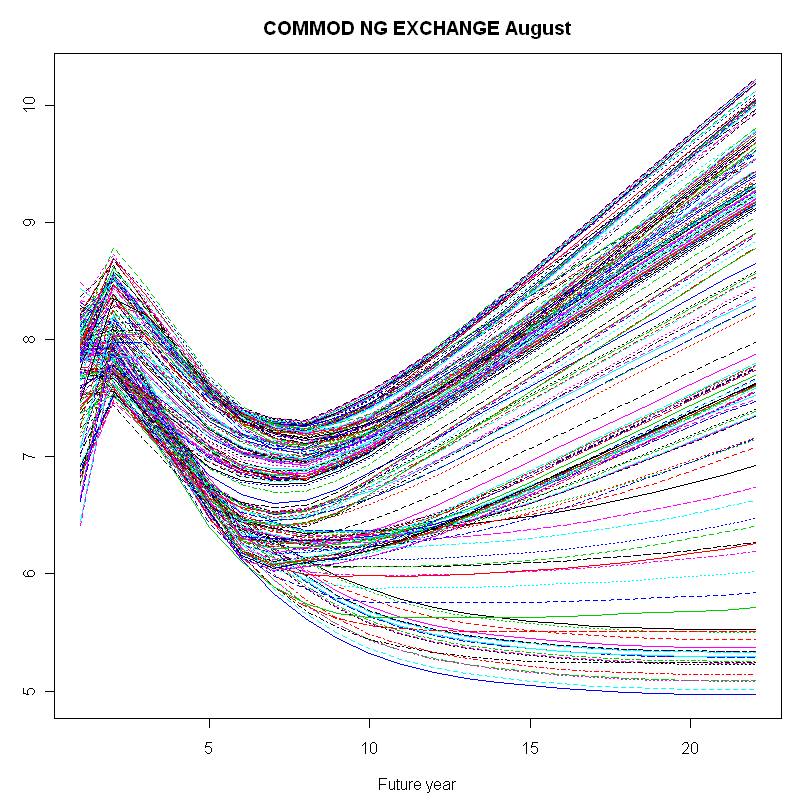
\includegraphics[height=2.5in]{figures/henry05.png}
\end{center}
}

\frame
{
\frametitle{NG EXCHANGE: Correlations among prices for different contracts}
\begin{center}
  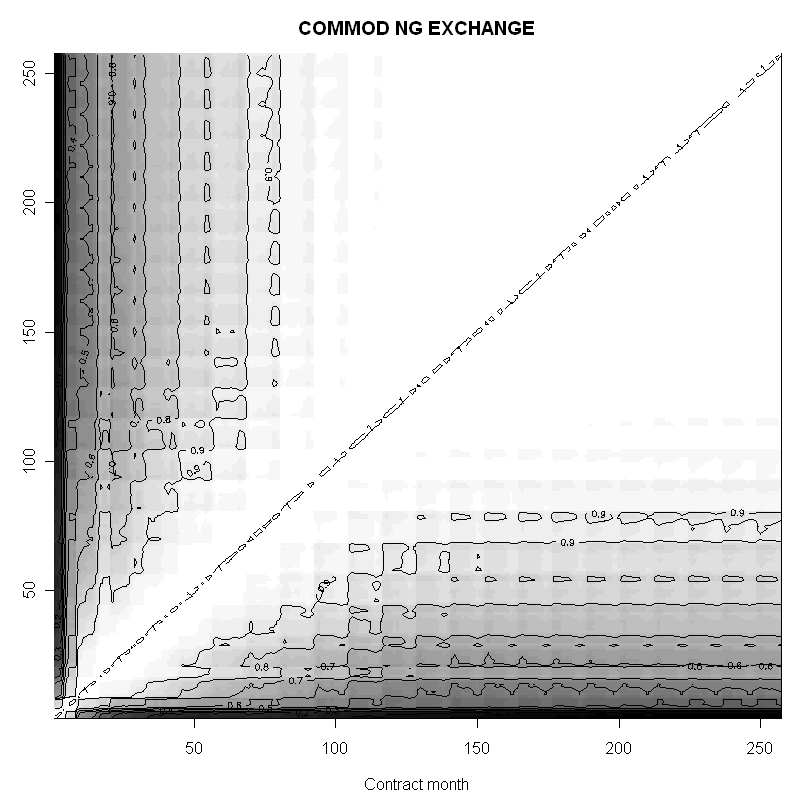
\includegraphics[height=2.5in]{figures/henry07.png}
\end{center}
}

%% now look at regional data
\frame
{
\frametitle{August 07 contracts, 17 regional reference curves}
\begin{center}
  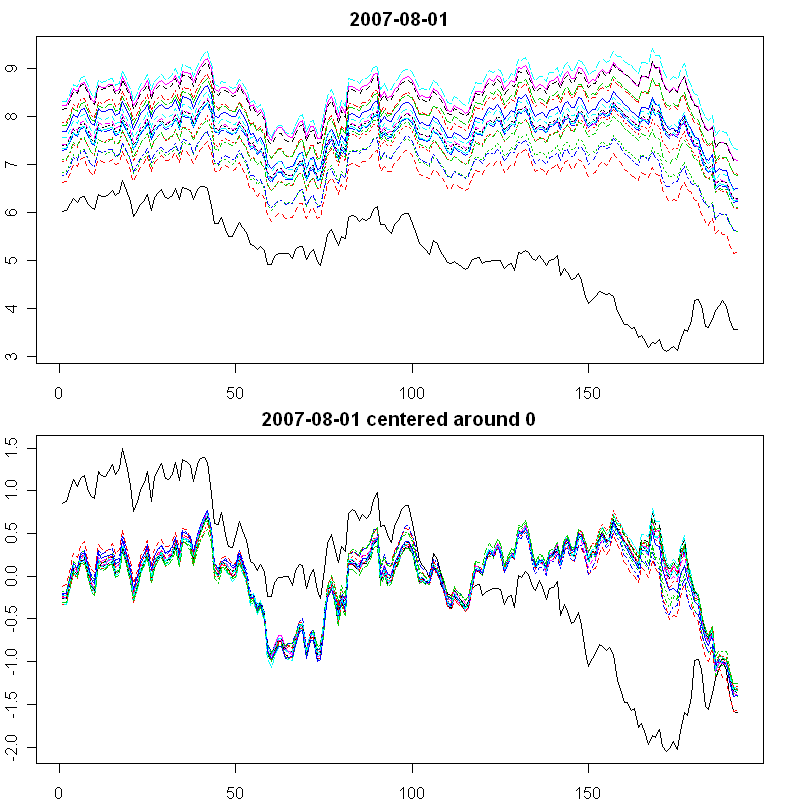
\includegraphics[height=2.5in]{figures/regional-0708-01.png}
\end{center}
}

\frame
{
\frametitle{Price correlation among 17 regional reference curves}
\begin{center}
  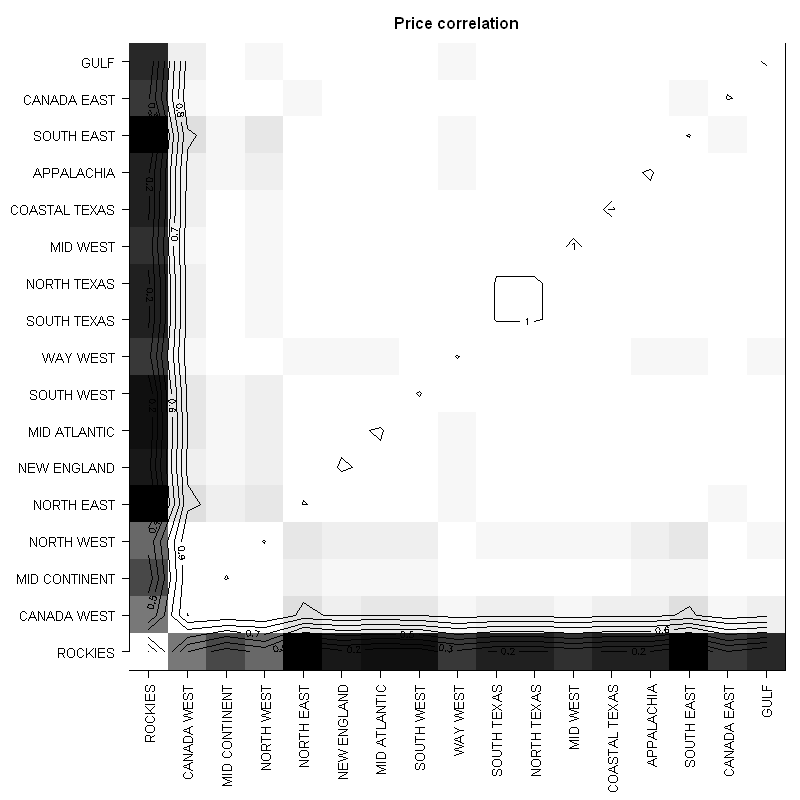
\includegraphics[height=2.5in]{figures/regional-0708-02.png}
\end{center}
}


\frame
{
\frametitle{Hierarchical clustering for  regional curves}
\begin{center}
  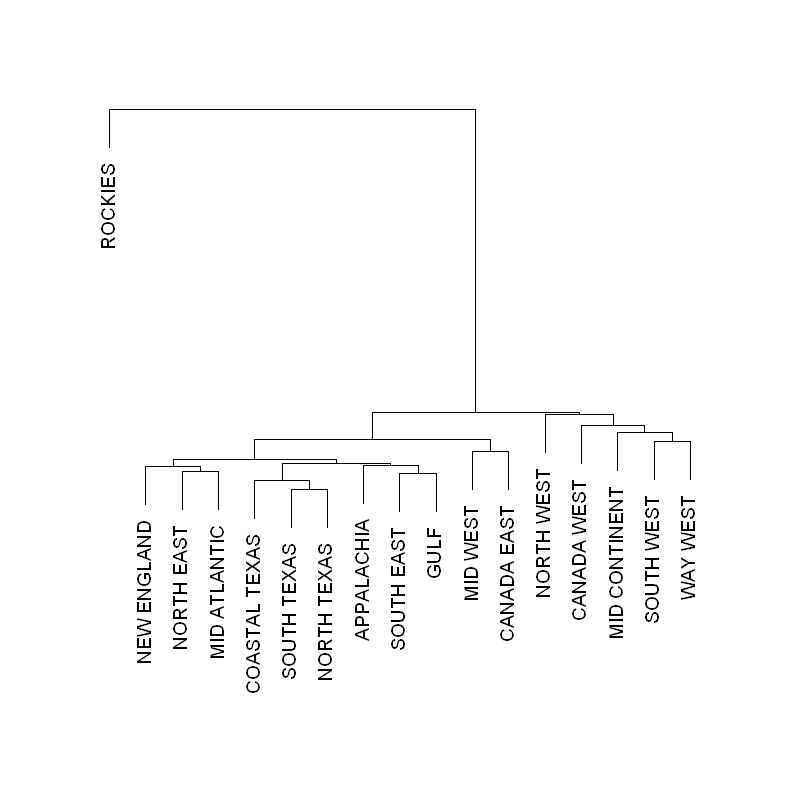
\includegraphics[height=3.0in]{figures/regional-0708-04.png}
\end{center}
}


%%%  Coal
\frame
{
  \frametitle{COL EXCHANGE historical prices}

\begin{center}
  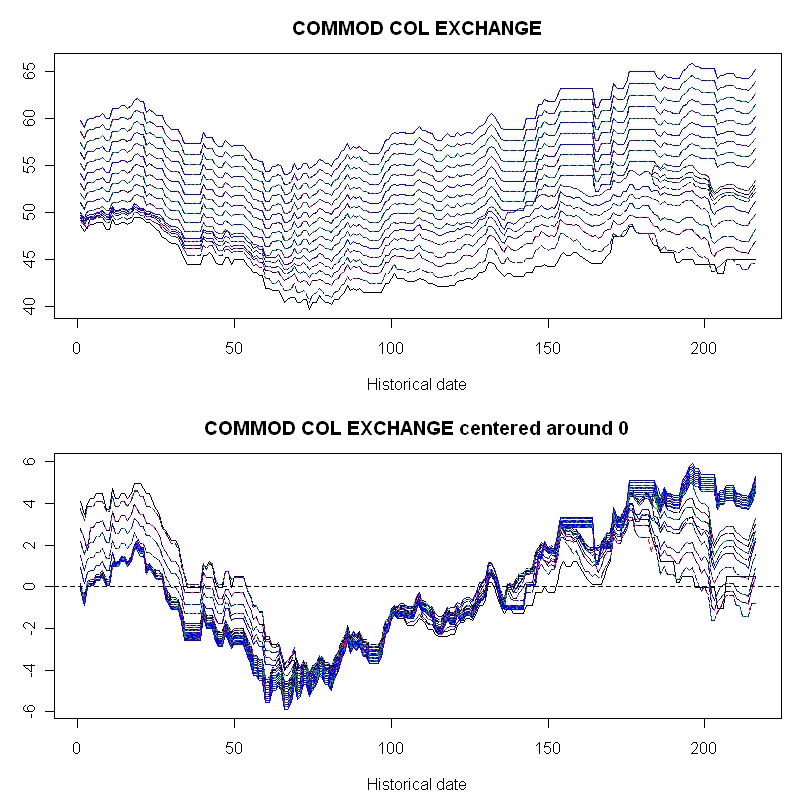
\includegraphics[height=2.5in]{figures/col01.png}
\end{center}
}

\frame
{
  \frametitle{COL EXCHANGE  prices by contract month}

\begin{center}
  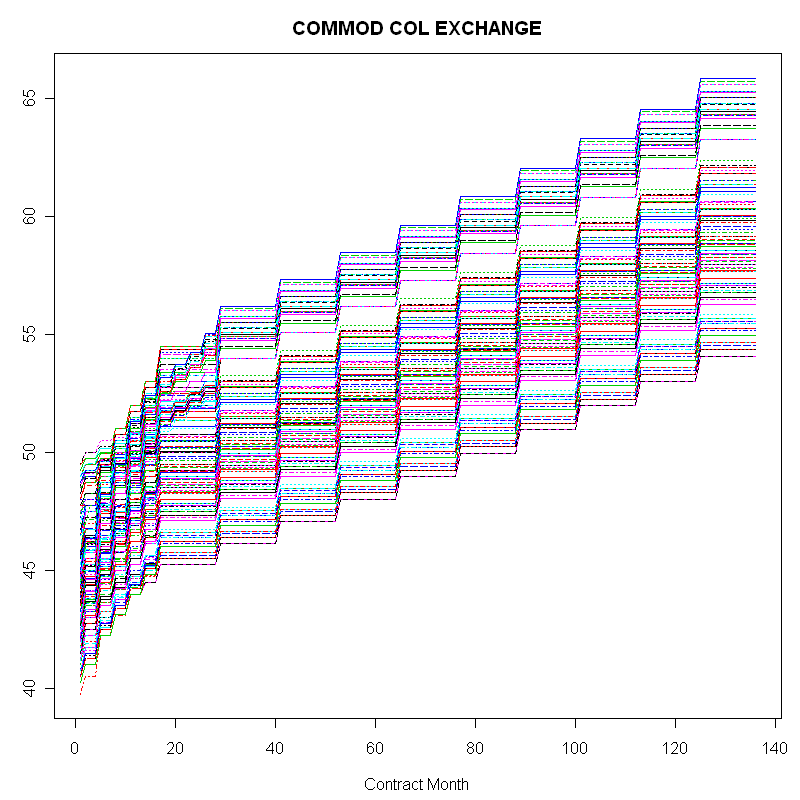
\includegraphics[height=2.5in]{figures/col02.png}
\end{center}
}

%%%  WTI
\frame
{
  \frametitle{WTI EXCHANGE historical prices}

\begin{center}
  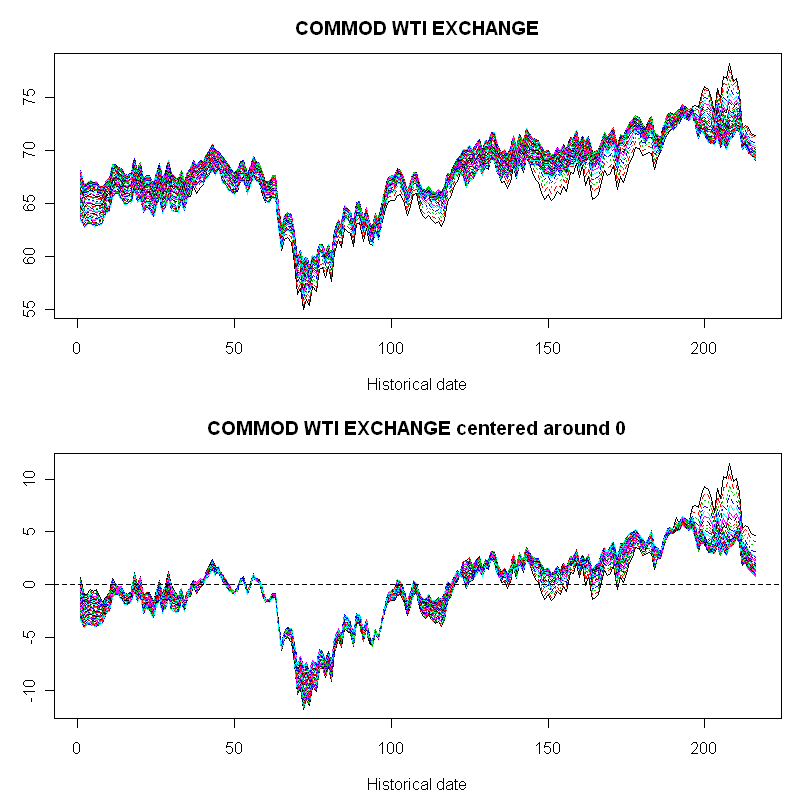
\includegraphics[height=2.5in]{figures/wti01.png}
\end{center}
}

\frame
{
  \frametitle{WTI EXCHANGE  prices by contract month}

\begin{center}
  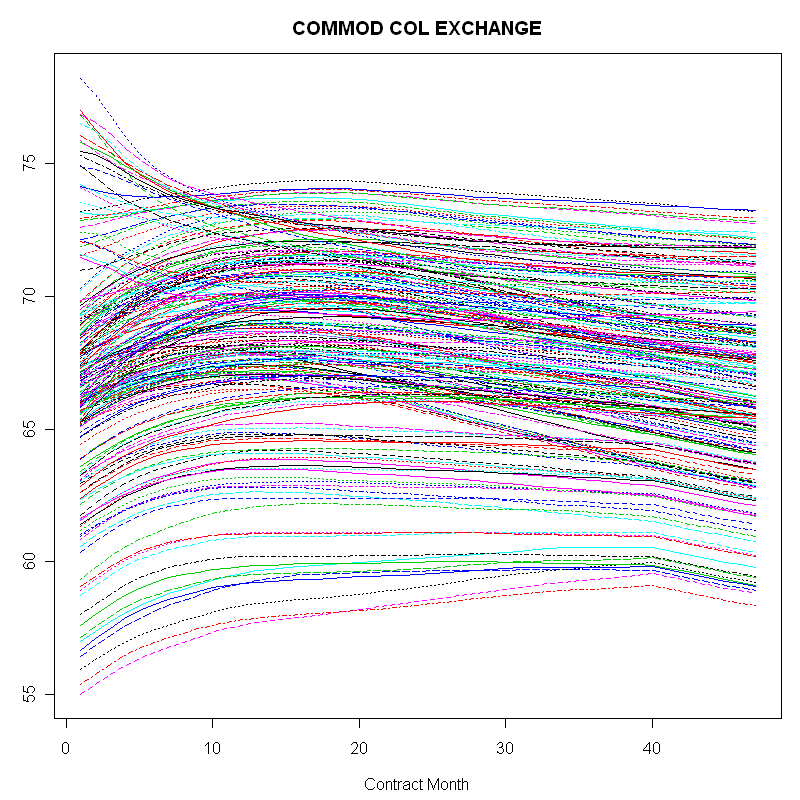
\includegraphics[height=2.5in]{figures/wti02.png}
\end{center}
}

%% three fuels
\frame
{
  \frametitle{Historical prices for three fuels}
\begin{center}
  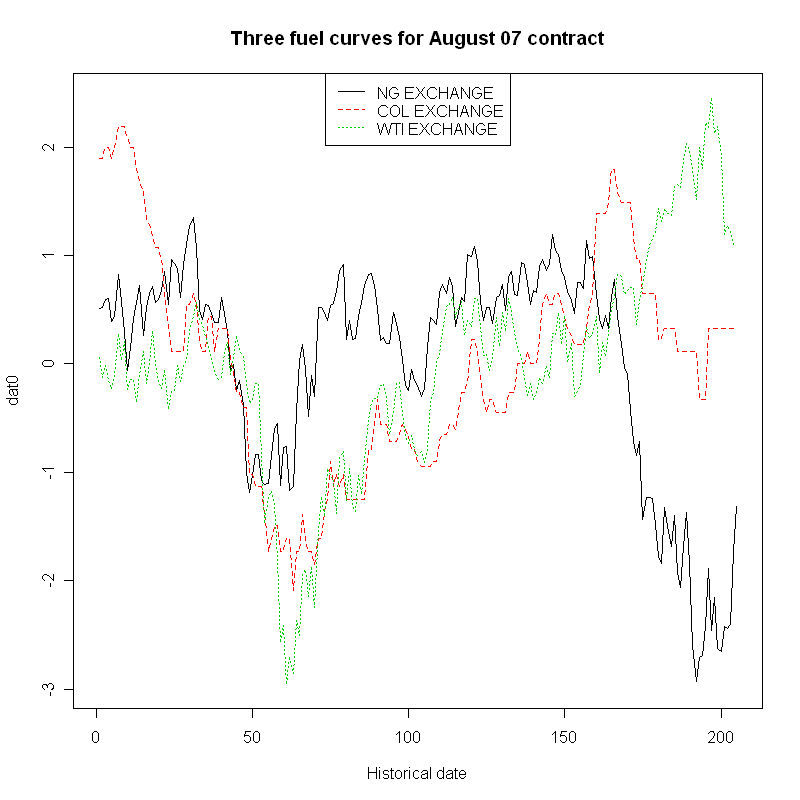
\includegraphics[height=2.5in]{figures/allfuels.png}
\end{center}
}

\frame{
  \frametitle{Findings}
\begin{itemize}
\item Curves are very similar.
\item Seasonality in NG, not COL/WTI
\item Three types of fuels are mildly correlated.
\end{itemize}
}

%%%%%%  power curves
\frame
{
  \frametitle{PWY 5X16 NYC historical prices}

\begin{center}
  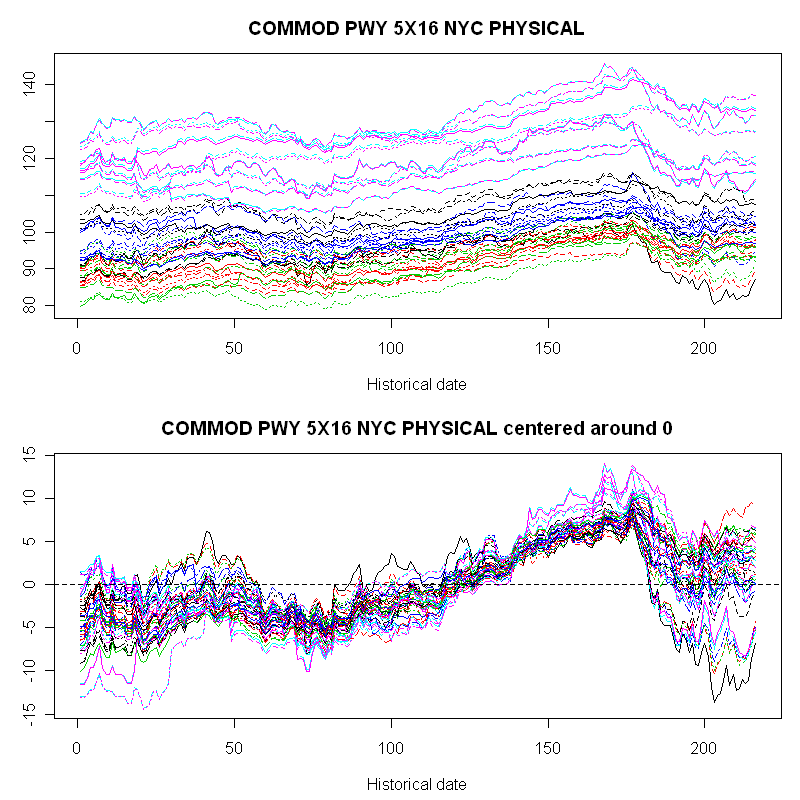
\includegraphics[height=2.5in]{figures/pwy01.png}
\end{center}
}

\frame
{
  \frametitle{PWY 5X16 NYC  prices by contract month}

\begin{center}
  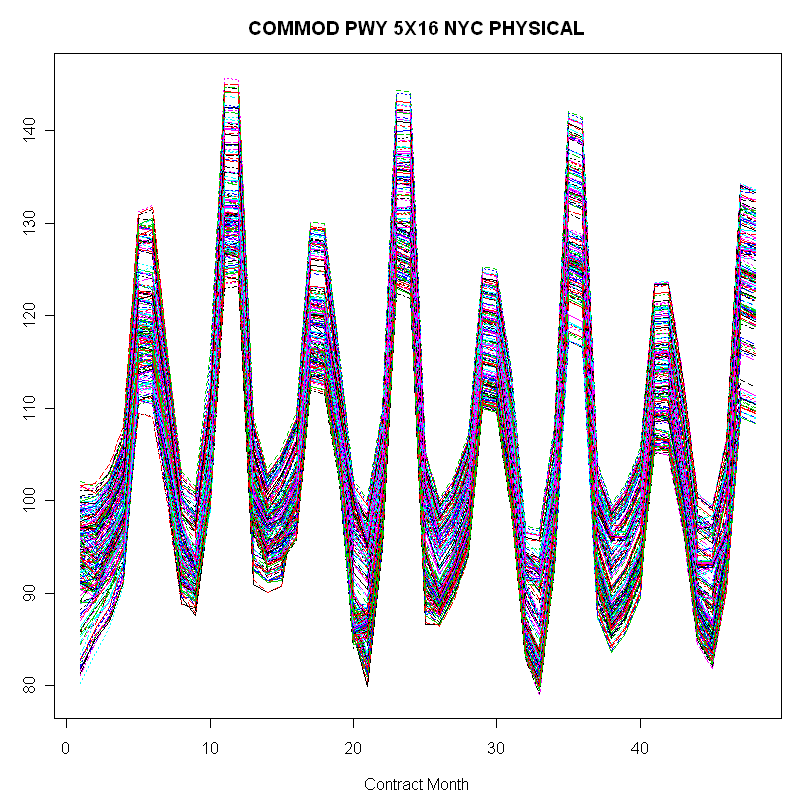
\includegraphics[height=2.5in]{figures/pwy02.png}
\end{center}
}

\frame
{
  \frametitle{All PWY curves for Sep 07 contracts}

\begin{center}
  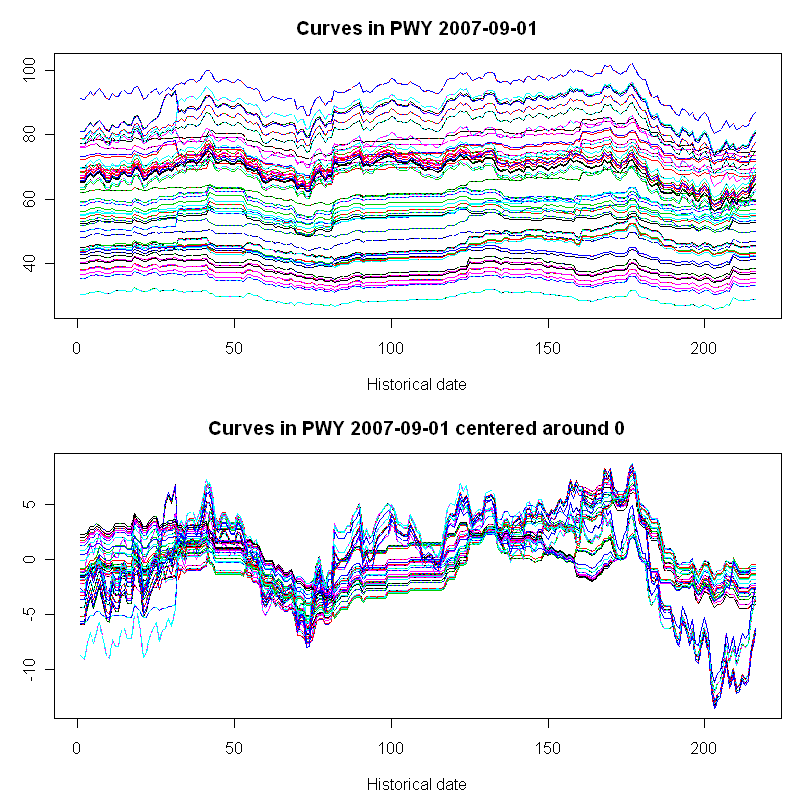
\includegraphics[height=2.5in]{figures/pwy-contract.png}
\end{center}
}

\frame
{
  \frametitle{K-means clustering on PWY curves, Sep 07}

\begin{center}
  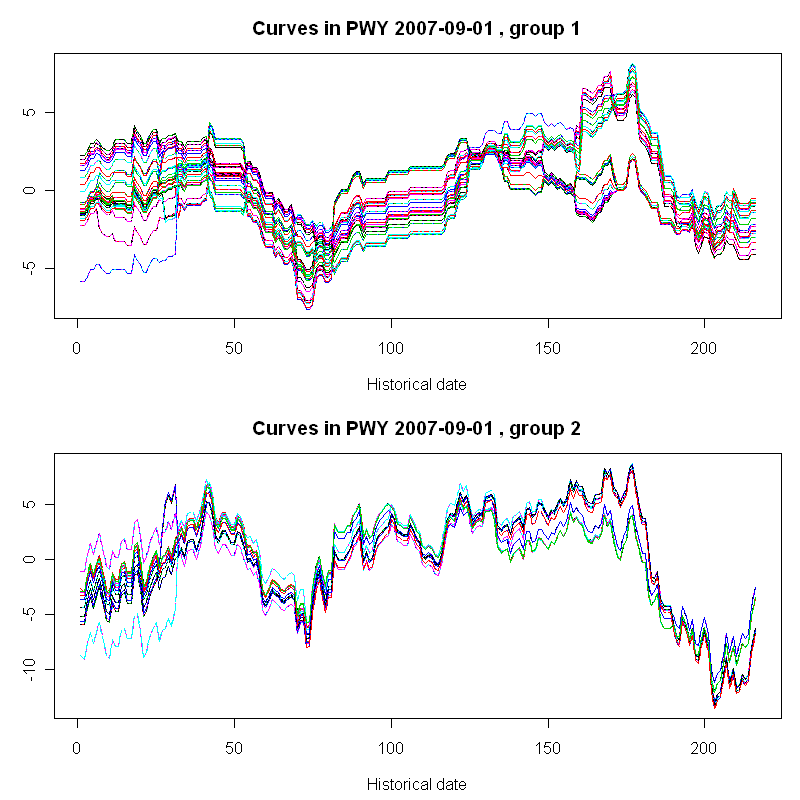
\includegraphics[height=2.5in]{figures/pwy-kmeans.png}
\end{center}
}

\frame
{
  \frametitle{PWY curve vs. Fuels}
\begin{center}
  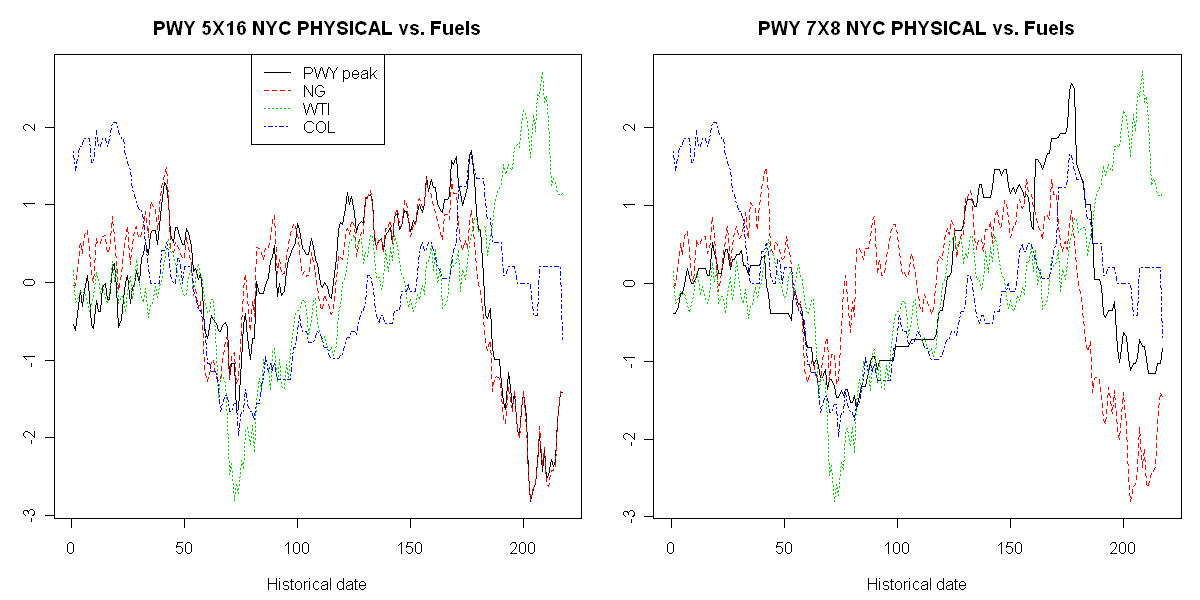
\includegraphics[height=2.0in]{figures/pwy-fuel.png}
\end{center}
}

\frame
{
  \frametitle{Correlation between PWY curves and Fuels, by contract month}

\begin{center}
  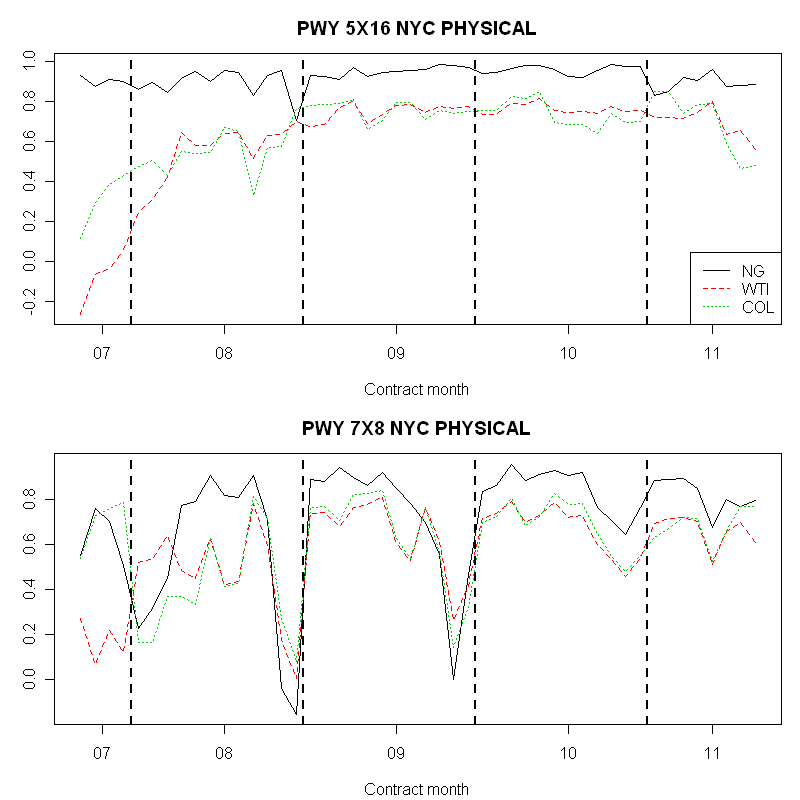
\includegraphics[height=2.5in]{figures/pwy-fuel-corr.png}
\end{center}
}

\frame
{
  \frametitle{Findings in electricity curves}
\begin{itemize}
\item For the same curve name, all contracts are similar.
\item For the same contract, curves are in groups.
\item Show Seasonality.
\item Correlated with fuels in different ways.
\end{itemize}
}


%%% Volatility
\frame
{
  \frametitle{Volatility - NG EXCHANGE}

\begin{center}
  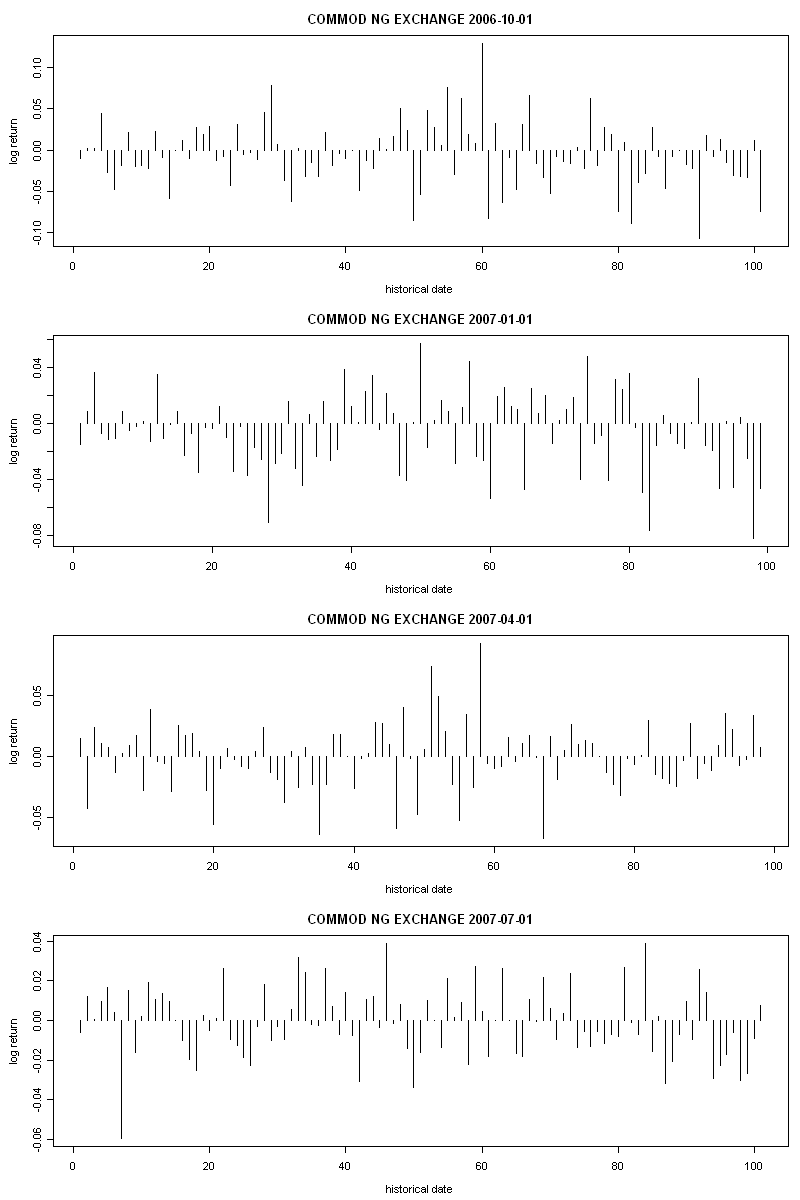
\includegraphics[height=2.5in]{figures/ng-exch-vol.png}
\end{center}
}

\frame
{
  \frametitle{Volatility - PWY NYC}

\begin{center}
  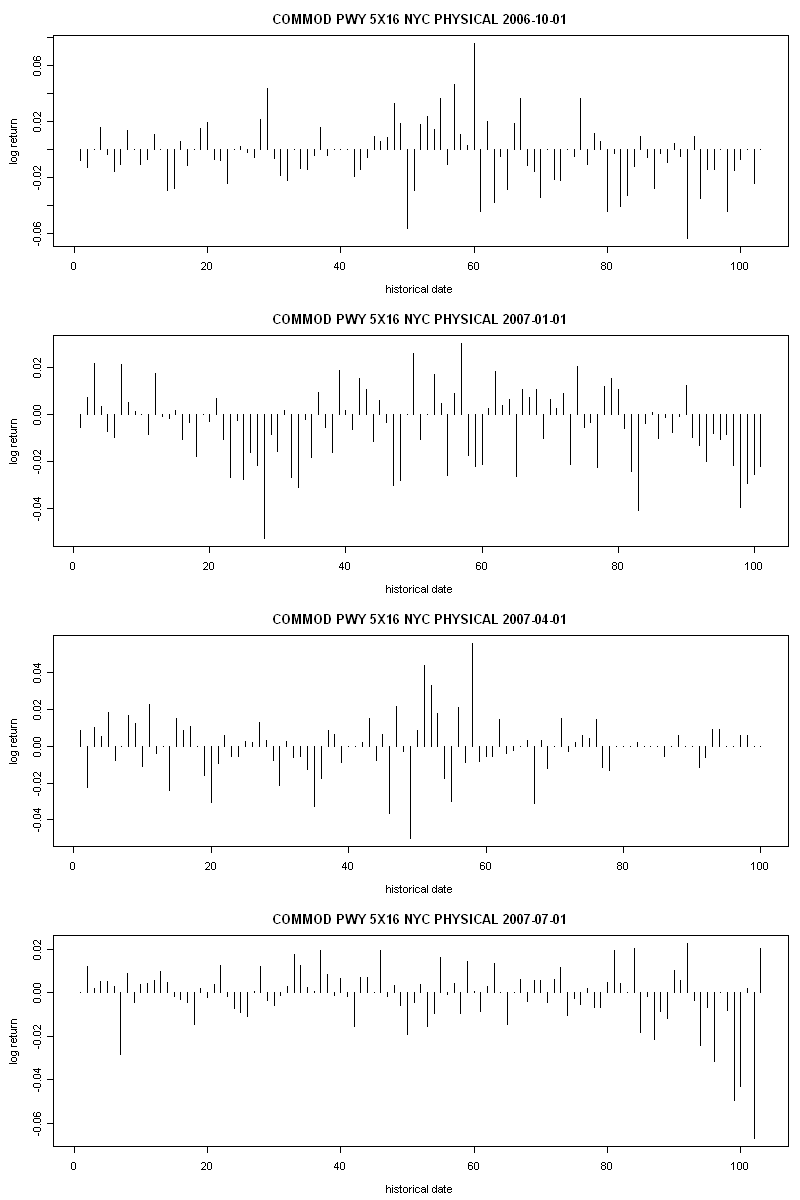
\includegraphics[height=2.5in]{figures/pwy-peak-vol.png}
  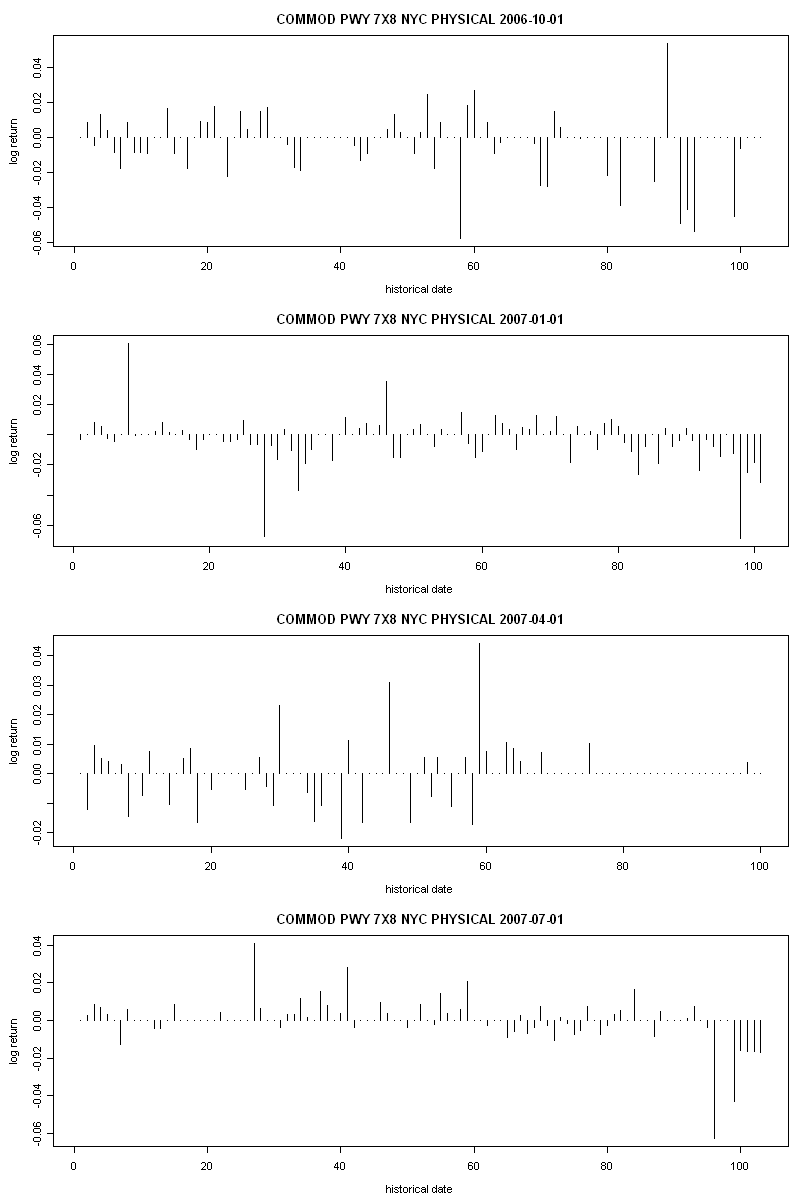
\includegraphics[height=2.5in]{figures/pwy-offpeak-vol.png}
\end{center}

}

\frame
{
  \frametitle{Volatility - PWJ WEST}

\begin{center}
  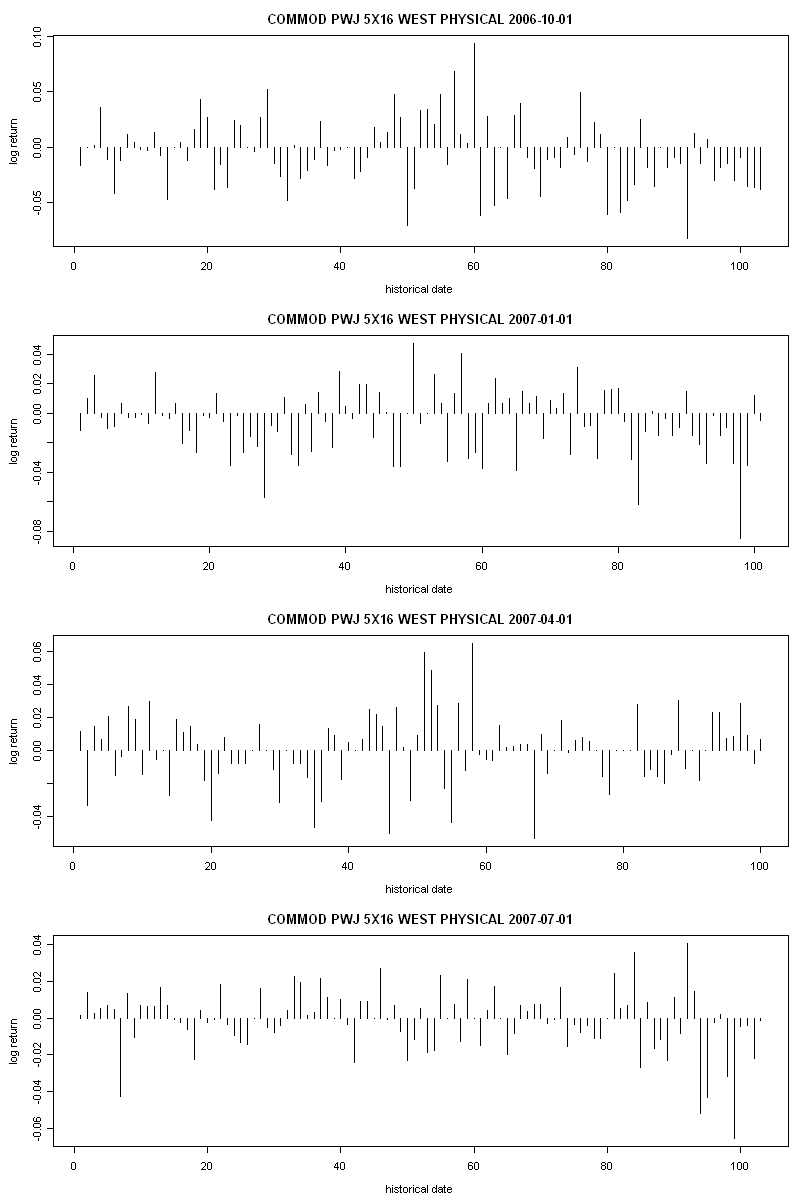
\includegraphics[height=2.5in]{figures/pwj-peak-vol.png}
  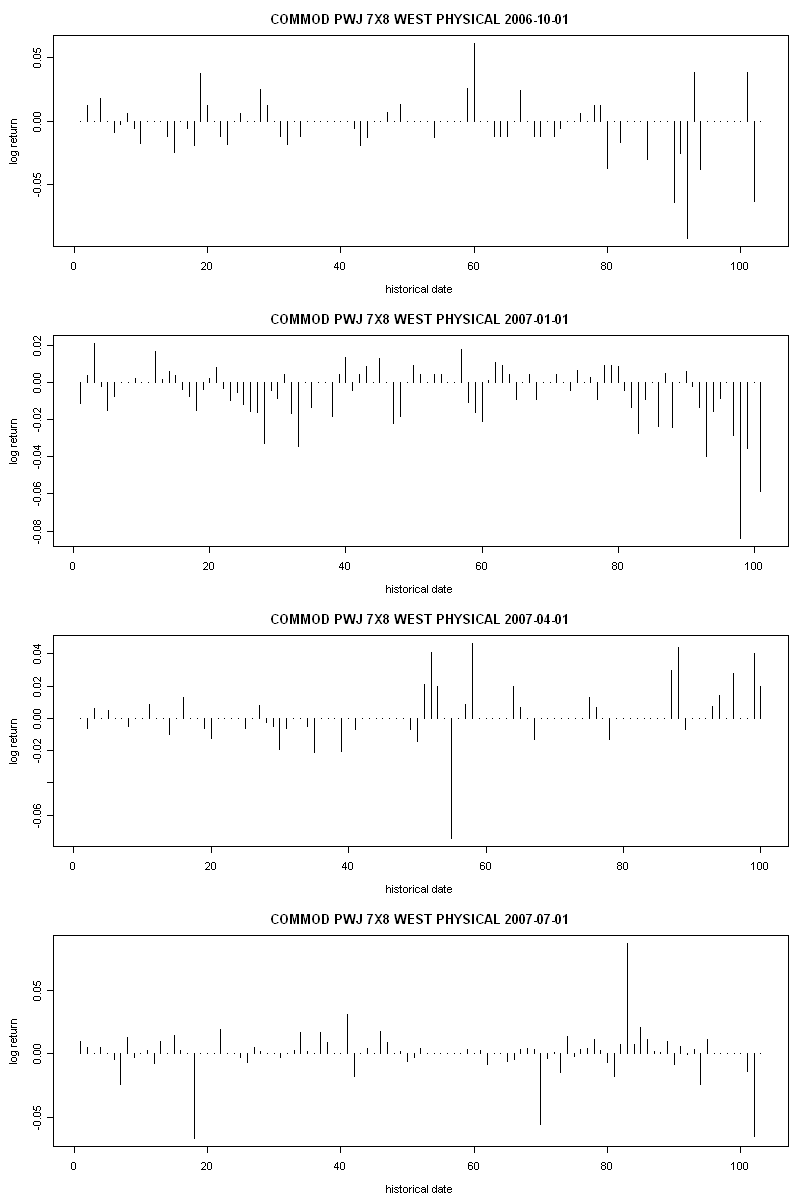
\includegraphics[height=2.5in]{figures/pwj-offpeak-vol.png}
\end{center}
}


\frame
{
  \frametitle{Findings}
\begin{itemize}
\item Volatilities for NG didn't change approaching maturity
\item Volatilities for power curves seem to increase 
for contracts in peak season??
\item Need more work to validate the findings.
\end{itemize}
}




%%%%%%%%%%%%%%%%%%%%%%%%%%%%%%%%%%%%%%%%%%%%%%%%
%% Method section
%%%%%%%%%%%%%%%%%%%%%%%%%%%%%%%%%%%%%%%%%%%%%%%%

\section{Method}

\frame
{
  \frametitle{Goals}
Our goal is to simulate forward prices for all curves in portfolio
(around 30,000).
\begin{itemize}
\item To simulate 30,000 correlated time series, dimension 
reduction (PCA) is needed. 
\item The result should be consistent with recent history.
\end{itemize}

\vspace{10pt}
Why not do PCA on everything? 
\begin{itemize}
\item PCA needs to work on the var/cov matrix (30,000 by 30,000).
\item Correlations are high among same types of commodities, 
relatively low between different types of commodities.
We will need many PCs to reasonably capture the variance.
\end{itemize}
}

\frame{
\frametitle{Our approach}
\begin{enumerate}
\item Took a hierarchical view on the data and built a curve pedigree. 
There are parents and children curves.
\item Use PCA for dimension reduction.
\item Simulate parents
correlatedly based on OU process assumption.
\item Simulated children based on simulated parents.
\end{enumerate}
}


%%%  PCA
\frame
{
  \frametitle{Principal Component Analysis (PCA)}
PCA can do:
\begin{itemize}
\item Orthogonalization: PCs are independent.
\item Dimension reduction: Most of the variances were captures by  a few PCs.
\end{itemize}

}

\frame
{
  \frametitle{PCA result on PWY 5X16 NYC}
The first 10 PCs of the historical prices 
(for 48 contracts and 200 historical days):
\begin{center}
  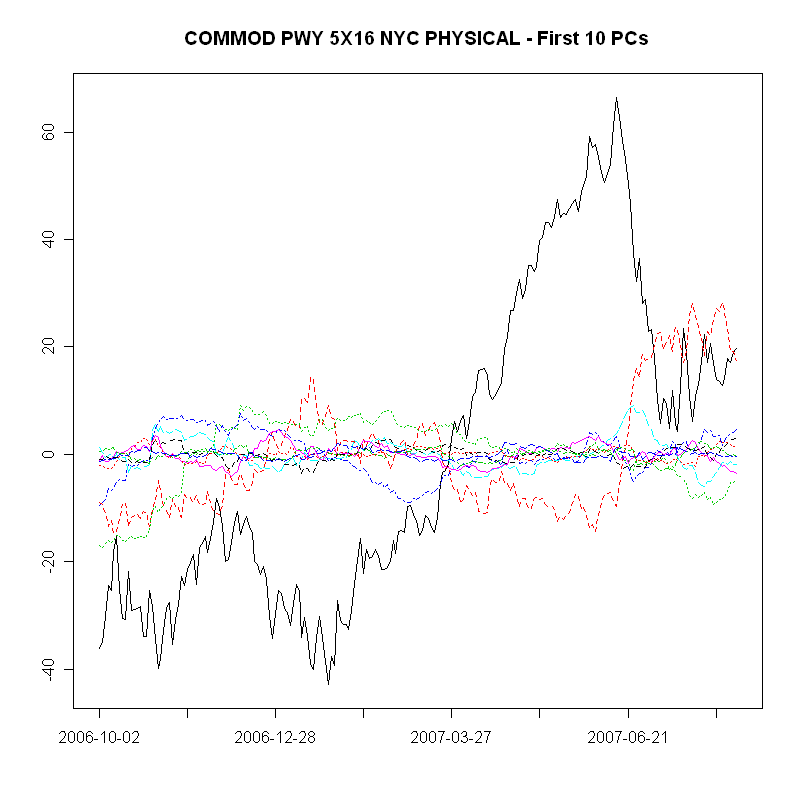
\includegraphics[height=2.3in]{figures/pc-pwy-peak.png}
\end{center}
}

\frame
{
  \frametitle{PCA result on PWY 5X16 NYC (cont.)}
Variance explained by the first 10 PCs:
\begin{table}[ht]
\begin{center}
\begin{tabular}{rrrrrr}
  \hline
 & PC 1 & PC 2 & PC 3 & PC 4 & PC 5 \\
  \hline
\% var  & 0.7962 & 0.1240 & 0.0424 & 0.0168 & 0.0083 \\
Cumulative \% var & 0.7962 & 0.9202 & 0.9625 & 0.9794 & 0.9877 \\
\hline \hline
 & PC 6 & PC 7 & PC 8 & PC 9 & PC 10 \\
\hline
\% var  & 0.0032 & 0.0018 & 0.0012 & 0.0010 & 0.0007 \\
 Cumulative \% var & 0.9909 & 0.9928 & 0.9939 & 0.9949 & 0.9956 \\
   \hline
\end{tabular}
\end{center}
\end{table}
}

%%%  curve pedigree
\frame
{
  \frametitle{Curve hierarchy}
\begin{itemize}
\item The hierarchy was made manually based on fundamentals.
\item Saved as a flat table in an Excel file. 
\item Program will read the file and do simulation.
\item User will have to maintain this until integration with other
IT projects.
\end{itemize}
}


\frame
{
  \frametitle{Curve hierarchy - Fuels}
\begin{itemize}
\item One commodity reference curve for each fuel type:
NG EXCHANGE, WTI EXCHANGE, COL NYMEX PHYSICAL.
\item NG curves were divided into 17 groups by region.
\item Each region has a regional reference curve.
  They are children of NG commodity reference curve.
\item Rest of the NG curves are children of regional reference curves
  respectively.
\item COL/WTI curves are children of their commodity reference curves.
\end{itemize}
}


\frame
{
  \frametitle{Curve hierarchy - Electricity}
\begin{itemize}
\item Two reference curves (peak and offpeak) for each electricity market.
They are children of WTI EXCHANGE, COL NYMEX PHYSICAL and the corresponding
NG regional reference curves.
\item Rest of the electricity curves are children of their corresponding
market reference curves.
\end{itemize}
}

\frame
{
  \frametitle{Curve hierarchy - Other market}
Other markets includes freight, emission, etc. At this time 
We didn't put any structure and these markets are simulated
independently. 

The hierarchy can be added easily by modifying the Excel file.
}

\frame
{
  \frametitle{Curve hierarchy illustration}
\begin{center}
  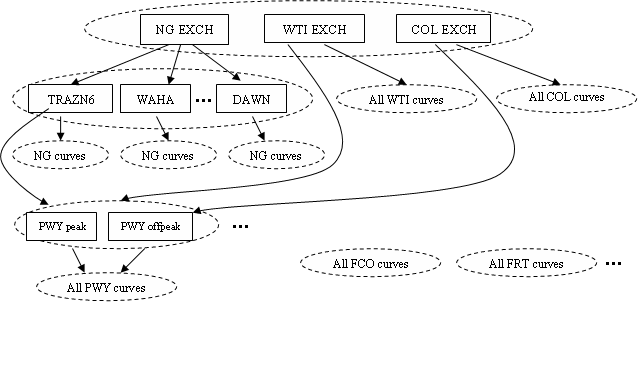
\includegraphics[height=2.5in]{figures/pedigree.png}
\end{center}
}

%%%  parents
\frame
{
  \frametitle{Simulating Parent Curves}
One crucial assumption is that {\color{red} log price} follows
OU process. For several curves their log prices
follow correlated OU processes. Simulation steps are:
\begin{itemize}
\item Do two rounds of PCA to break the correlations
among contracts and curves. 
Resulting PCs (linear transformation of log prices)
are uncorrelated OU processes.
\item Estimate OU parameters from historical then simulate
forward PCs. 
\item Transform back to original scale.
\end{itemize}
}

\frame
{
  \frametitle{Simulating Parent Curves  (cont.)}
What if OU assumption fails? 

\vspace{10pt}
Currently we make up some numbers for parameters. 
This isn't too bad. 
\begin{itemize}
\item Results are approximately GBM.
\item Weak force pulling price back to historical median.
\end{itemize}

\vspace{10pt}
Potentially we can do:
\begin{itemize}
\item Use HMM to divide historical into ``up'', ``down'', ``flat''
periods. Estimate transition/emission probability.
\item Remove trend and model residuals as OU. 
\item Simulate both trend and residuals.
\end{itemize}
}

%%%  children
\frame
{
  \frametitle{Simulating Children Curves}
Children curves were correlated to their parents through regression.

\vspace{15pt}
Notations for next a few slides are:
\begin{itemize}
\item $y(t)$: log historical prices of the child curve for day $t$, 
\item $\Delta y(t)$: log return of the child curve on day $t$. 
\item $x_p(t)$: log historical prices of the $p^{th}$ parent curve for day $t$, 
$p=1, 2, \ldots, P$.
\item $\Delta x_p(t)$: log return of the $p^{th}$ parent for day $t$, 
\end{itemize}

The following several models were considered. 
}


\frame
{
  \frametitle{Regression of log prices (Model 1)}

Regress child's log price on parents' log prices:
\begin{equation}
y(t)=\beta_0 + \sum_{p=1}^P \beta_p x_p(t) + \epsilon(t).
\label{model1}
\end{equation}
Problems are:
\begin{itemize}
\item ``Spurious'' regression so $R^2$ is not reliable
\item Assuming children prices change with parents 
on a daily basis, which isn't necessarily true.
\item $\epsilon(t)$ auto-correlated, hard to simulate.
\end{itemize}
}

\frame
{
  \frametitle{Regression of log returns (Model 2)}
Regress child's log return on parents' log return:
\begin{equation}
\Delta y(t)=\beta_0 + \sum_{p=1}^P \beta_p \Delta x_p(t) + \epsilon(t).
\label{model2}
\end{equation}
Problems are:
\begin{itemize}
\item Fitting is poor  with $R^2$ dropped to below 0.5.
\item Child and parents are co-integrated processes: 
prices roughly track each other, but not on daily basis.
\end{itemize}
}

\frame
{
  \frametitle{Another regression model (Model 3)}
Model \ref{model2} can  be written as:
\[ y(t)=\beta_0 + y(t-1) + \sum_{p=1}^P \beta_p [x_p(t)-x_{p}(t-1)] + \epsilon(t). \]
It regresses child's today's price on
its previous day's price  and parents' today
and previous day's prices, with constrains on the coefficients. 
\vspace{15pt}
We removed the constrains and came up with:
\begin{equation}
  y(t)=\beta_0 + \beta_1 y(t-1) +
\sum_{p=1}^P [\beta_{p1} x_p(t) + \beta_{p2} x_p(t-1) ] + \epsilon(t).
\label{model3}
\end{equation}
}


\frame
{
  \frametitle{Model 3 (cont.)}
Connection between Model \ref{model3} and regression on log prices:
\begin{itemize}
\item After regression on log price, do another regress on residuals:
$\epsilon(t) \sim \epsilon(t-1)$. The residuals show little AC.
\item The residual regression is similar to our model 
(with 1 less degree of freedom). 
\end{itemize}
}

\frame
{
  \frametitle{Model 3 (cont.)}
There's connection between Model \ref{model3} and Error Correction Model (ECM)
for co-integrated processes. 

\begin{itemize}
\item From our model, we can get:
\[\Delta y(t) = \beta_1 \Delta y(t-1) +
\sum_{p=1}^P [\beta_{p1} \Delta x_p(t) + \beta_{p2} \Delta x_p(t-1)] +
\Delta \epsilon(t). \]
\item ECM doesn't have $\Delta x_p(t)$ because they don't assume to know
it beforehand. 
\item Our model is more liberal.
\end{itemize}
}

\frame
{
  \frametitle{Final model}
Note that the input of children curve simulation are PCs 
so they were centered around 0. We remove the intercept
in regression and came up with our final model:
\begin{equation}
  y(t)=\beta_1 y(t-1) +
\sum_{p=1}^P [\beta_{p1} x_p(t) + \beta_{p2} x_p(t-1) ] + \epsilon(t).
\label{model4}
\end{equation}

\begin{itemize}
\item Model selection procedure was used to select parents. 
\item Fitting is good with high $R^2$
\item No auto-correlation in residuals
\end{itemize}
}


\frame
{
  \frametitle{Some details}
There are some details in simulating children curves:
\begin{enumerate}
\item Children curves in the same group (market) are 
simulated together to keep the correlation in 
residual processes $\epsilon(t)$. What's the correlation
among $\epsilon(t)$?
\begin{itemize}
\item Correlation among estimated residuals underestimate
the truth because children are co-integrated. 
\item I'm using the correlation in log prices $y(t)$. 
\end{itemize} 

\item For different forward time step, should 
residuals $\epsilon(t)$ form the same distribution?
\begin{itemize}
\item Yes. $\epsilon(t)$
can be (kind of) viewed  as the co-integrated
process of the child and parent curves, so it should be
stationary.
\end{itemize} 

\end{enumerate}
}

%%%%%%%%%%%%%%%%%%%%%%%%%%%%%%%%%%%%%%%%%%%%%%%%
%% result section
%%%%%%%%%%%%%%%%%%%%%%%%%%%%%%%%%%%%%%%%%%%%%%%%

\section{Results}

\frame
{
  \frametitle{Simulation settings}
\begin{itemize}
\item Use 300 historical days to predict future.
Exclude the weekends and holidays there are around 210
historical pricing days.
\item Use 5 principal components to represent both the curves
and the months. This will capture over 95\% of the variance in data
most of the time.
\item Simulate daily until the end of next month, then do monthly
for another 46 months. Totally there are around 80 forward time points.
\item Simulation was done for contracts of 48 future months.
\item Generate 1000 independent simulations.
\end{itemize}

}

%%%  single curve
\frame
{
  \frametitle{Simulation result for NG EXCHANGE}
Daily forward prices for four future contracts:
\begin{center}
  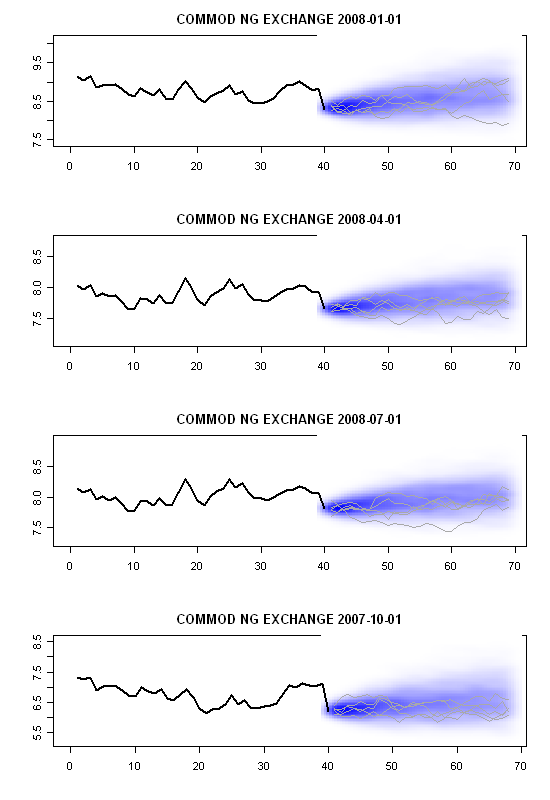
\includegraphics[height=2.5in]{figures/ng-exchange-allsim.png}
\end{center}
}

%%%  single curve
\frame
{
  \frametitle{Simulation result for NG EXCHANGE (cont.)}
Monthly forward prices for four future contracts:
\begin{center}
  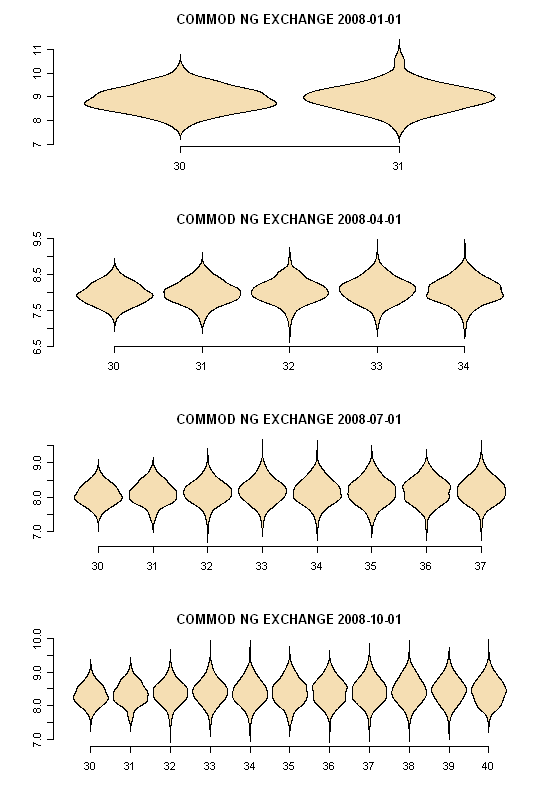
\includegraphics[height=2.5in]{figures/ng-exchange-violin.png}
\end{center}
}

\frame
{
  \frametitle{Simulation result for NG EXCHANGE (cont.)}
All contracts, one simulation:
\begin{center}
  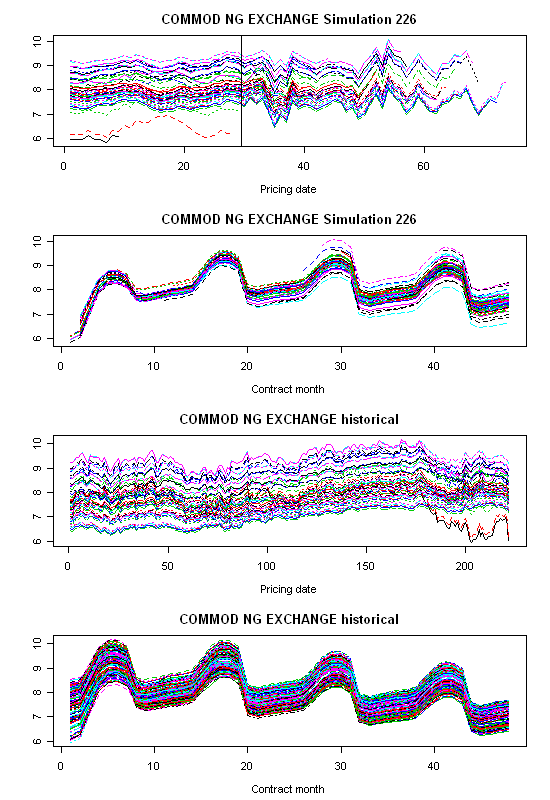
\includegraphics[height=2.5in]{figures/ng-exchange-allmon.png}
\end{center}
}



\frame
{
  \frametitle{Volatility}
Historical vs. simulated  volatility for NG EXCHANGE. 
\begin{table}[htbp]
\begin{center}
\begin{tabular}{r|rrrrrr}
\hline
& & 9/07 & 10/07 & 11/07 & 12/07 & 1/08 \\
  \hline
  \multirow{2}{*}{Daily} & 
  Hist & 0.0228 &  0.0185 &   0.0154 &  0.0144 &  0.0142  \\
 & Sim & 0.0245 &   0.0194 &   0.0154 &  0.0142  & 0.0139 \\ \hline \hline
  \multirow{2}{*}{Weekly} & 
  Hist & 0.0423 &   0.0347 & 0.0291 &  0.0275 &  0.0271 \\
   & Sim & 0.0519 &   0.0390 &   0.0303 &  0.0273 &   0.0267 \\ \hline \hline 
  \multirow{2}{*}{Biweekly} & 
  Hist & 0.0557  & 0.0452 &   0.0378 &   0.0362 &   0.0358 \\
  & Sim & 0.0409 &   0.0356 &   0.0284 &   0.0258 &   0.0254  \\
   \hline
\end{tabular}
\end{center}
\label{tbl-ng-vol}
\end{table}
}


\frame
{
  \frametitle{Volatility (cont.)}
\begin{itemize}
\item Daily volatilities are usually accurate.
\item Long term volatilities are very curve dependent. 
\item When it fails, it's likely that the OU assumption was incorrect,
or unstable. Other process assumption worth trying. 
\end{itemize}
}

%% heat content
\frame
{
  \frametitle{Simulated vs. historical heat content}
Heat content for PWY 5X16 NYC PHYSICAL
\begin{center}
  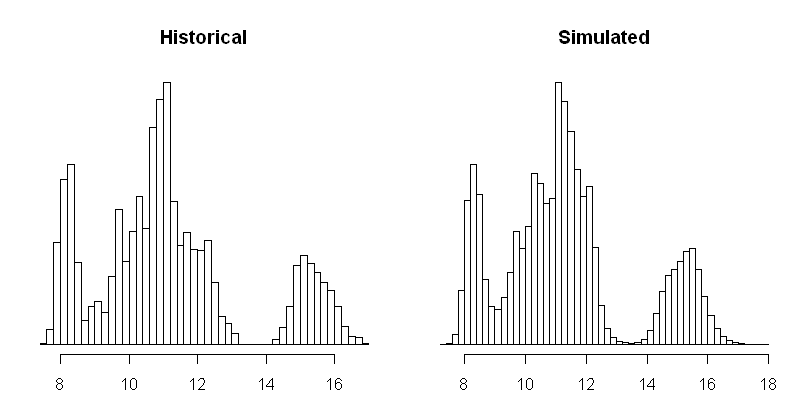
\includegraphics[height=2.0in]{figures/heatcontent.png}
\end{center}


}

%%% multiple curve correlations
\frame
{
  \frametitle{Simulation results for multiple curves}
One simulation for three NG curves:
\begin{center}
  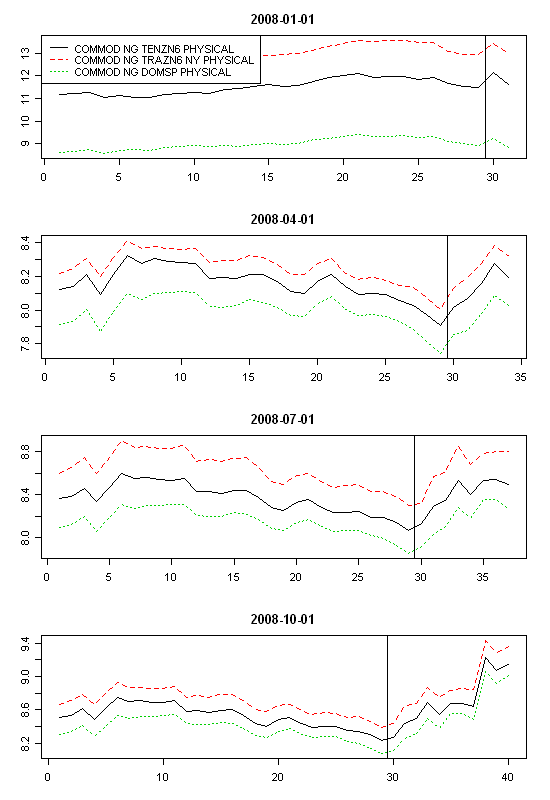
\includegraphics[height=2.5in]{figures/ng-multicurve.png}
\end{center}


}

\frame
{
Historical vs. simulated correlations among three NG curves:
  \frametitle{Correlations in simulated curves}
\begin{table}[htbp]
\begin{center}
\begin{tabular}{rrrr}
  \hline
 &  \multicolumn{3}{c}{Historical}  \\ \hline
 & TENZN6  & TRAZN6 NY  & DOMSP    \\
  \hline
TENZN6  & 1.0000 & 0.9988 & 0.9983  \\
  TRAZN6 NY  & 0.9988 & 1.0000 & 0.9976  \\
  DOMSP  & 0.9983 & 0.9976 & 1.0000  \\
   \hline \hline
   &  \multicolumn{3}{c}{Simulated} \\ \hline
   TENZN6  & 1.0000 & 0.9737 & 0.9640 \\
   TRAZN6 & 0.9737 & 1.0000 & 0.9763 \\
   DOMSP & 0.9640 & 0.9763 & 1.0000 \\
   \hline
\end{tabular}
\end{center}
\label{tbl-ng-cor}
\end{table}
}


\frame
{
  \frametitle{Simulation results for multiple curves}
One simulation for three electricity curves in different markets 
(prices were shifted and scaled):
\begin{center}
  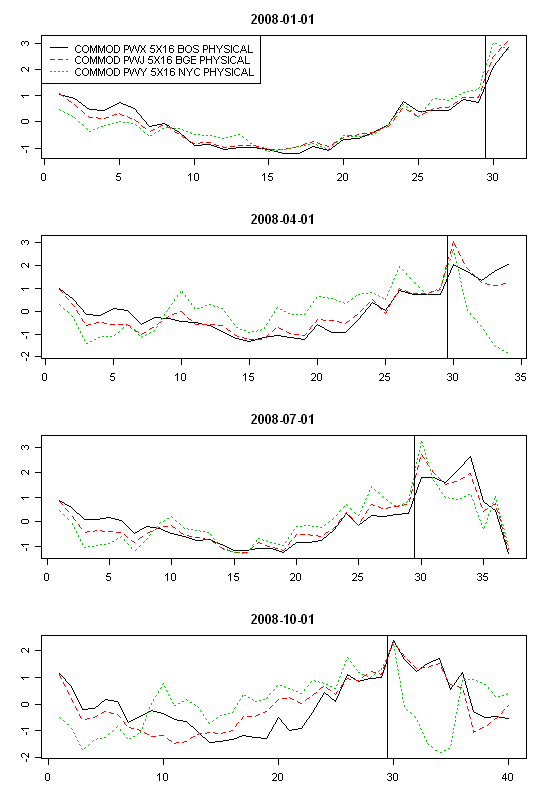
\includegraphics[height=2.5in]{figures/elec-multicurve.png}
\end{center}

}

\frame
{
  \frametitle{Correlations among simulated curves}
Historical vs. simulated correlations among three electricity curves:
\begin{table}[htbp]
\begin{center}
\begin{tabular}{rrrr}
\hline
 &  \multicolumn{3}{c}{Historical} \\  \hline
 &  5X16 BOS  &  5X16 BGE  &  5X16 NYC  \\
  \hline
 5X16 BOS  & 1.0000 & 0.8643 & 0.9293  \\
   5X16 BGE  & 0.8643 & 1.0000 & 0.9414  \\
   5X16 NYC  & 0.9293 & 0.9414 & 1.0000  \\
   \hline \hline
  & \multicolumn{3}{c}{Simulated} \\ \hline
   &  5X16 BOS  &  5X16 BGE  &  5X16 NYC  \\
  5X16 BOS & 1.0000 & 0.8052 & 0.8205 \\
  5X16 BGE & 0.8052 & 1.0000 & 0.8813 \\
  5X16 NYC  & 0.8205 & 0.8813 & 1.0000 \\ \hline
\end{tabular}
\end{center}
\label{tbl-elec-cor}
\end{table}
}

\frame
{
The correlations among simulated curves in different market
were underestimated. Why??
Because we correlate them through their parents.

\vspace{20pt}
To show this, let $X$, $Y$, $Z$ be random variables with
$cor(X,Y)=\rho_1$, $cor(Y,Z)=\rho_2$.
What's the minimum value of $\rho=cor(X,Z)$ 
when $\rho_1$ and $\rho_2$ are sufficiently large, say, 0.8?
}

\frame {
Correlation is projection. So
$\rho \ge cos[cos^{-1}(\rho_1)+cos^{-1}(\rho_2)]$.
\begin{itemize}
\item $\rho_1=\rho_2=0.99 \Rightarrow \rho \ge 0.96$, 
this is the case for NG curves. 
\item $\rho_1=\rho_2=0.90 \Rightarrow \rho \ge 0.62$,
this is the case for electricity curves.
\end{itemize}

\vspace{20pt}
Potential solutions are:
\begin{itemize}
\item Further divide regions into smaller subregions.
\item Use more parent curves.
\end{itemize}
}


\frame
{
  \frametitle{Implementation}
\begin{itemize}
\item Software was written in open source statistical 
programming language {\tt R}.
\item One run takes 3 hours on a single PC (2.8GHz, 2G RAM).
\item Parallelly distributed using {\tt Condor} (John).
\end{itemize}
}

%%%%%%%%%%%%%%%%%%%%%%%%%%%%%%%%%%%%%%%%%%%%%%%%
%% Future works
%%%%%%%%%%%%%%%%%%%%%%%%%%%%%%%%%%%%%%%%%%%%%%%%

\section{Future Works}

%%%  single curve
\frame
{
  \frametitle{Future Works}
\begin{enumerate}
\item Stochastic process assumption.
\begin{itemize}
\item Currently use OU process but 
other models can be plugged in easily.
\item Use HMM to simulate trend?
\end{itemize}
\item Curve dependency: talk to the traders.
%\end{itemize}
%}

%\frame
%{
%  \frametitle{Future Works (cont.)}
%\begin{itemize}
\item Nonlinear dimension reduction (LLE): use a few
components to capture nonlinearity in the data.
\begin{itemize} 
\item Nonlinearity in data is not obvious.
\item Involves many other calculations. 
The computational gain is doubtful.
\end{itemize}

\item Modeling volatility: this is difficult.
\item Econometrics models? 
\end{enumerate}

}

%%%%%%%%%%%%%%%%%%%%%%%%%%%%%%%%%%%%%%%

\frame
{
  \frametitle{Acknowledgment}
\begin{itemize}
\item Adrian
\item Aram
\item John
\item Haibin
\item Sailesh
\item Leyu, Pramod and Aristide
\item Karl, Rafa and other professors in Hopkins
\item Shijie 
\item The audience
\end{itemize}

}


\end{document}
